\documentclass[12pt]{article}

\usepackage[bottom]{footmisc}
\usepackage[margin=2cm]{geometry} 
\usepackage[shortlabels]{enumitem}
\usepackage[italicdiff]{physics}
\usepackage[at]{easylist}
\usepackage[normalem]{ulem}
\usepackage{amssymb,amsmath,amsthm,verbatim,graphicx}
%\usepackage{stmaryrd,mathtools} % extra symbols
%\usepackage{derivative,braket} % some alternatives to physics
\usepackage{hyperref} % for links
%\usepackage[compat=1.18]{pgfplots} % for plots
%\usepackage{minted,xcolor} % for linting
%\setminted{baselinestretch=0.75,style=gruvbox-light,fontsize=\small,fontfamily=courier,linenos}
\usepackage{csvsimple}
\usepackage{subcaption}

\renewcommand{\epsilon}{\varepsilon}
\renewcommand{\theta}{\vartheta}
\renewcommand{\phi}{\varphi}

\renewcommand{\L}{\mathcal{L}}

\newcommand{\N}{\mathbb{N}}
\newcommand{\Z}{\mathbb{Z}}
\newcommand{\Q}{\mathbb{Q}}
\newcommand{\R}{\mathbb{R}}
\newcommand{\C}{\mathbb{C}}

\newcommand{\epsn}{\epsilon_0}
\newcommand{\units}[1]{\ \mathrm{#1}}

\title{PHYS 3330 Final Project Proposal: 4-bit Digital Multiplier}

\author{Elijah Christie, Lev Kryvenko}

\date{October 26, 2026}

\begin{document}

\maketitle

\section{Project Outline}
\subsection{Description}
On a high level, we plan to build a circuit that takes two 4-bit numbers and multiplies them using pure logic. This will be done using only elementary logic gates, there will be a total of 64 logic gates in this circuit. To interface with this circuit, we will use two dip switches for input. Then finally an Arduino will take the inputs and outputs and display each on 7-segment displays.

The circuit does not have an analog core as suggested in the project guidelines. But this idea of manually implementing a multiplier using only logic gates really captivated us, so we hope that the complexity of our circuit makes up for it being completely digital at its core. Also, our use of the Arduino is limited to the displays---we are not using it at any point for the core logical circuit.

\subsection{Core Logical Multiplier Circuit}
We have designed and validated a design for the internal circuit in LTSpice. While we will not use half-adder or full-adder gates in the actual circuit, we implemented them as parts in LTSpice for simplicity of designing the actual multiplier. Their schematics can be seen in \autoref{fig:adders}.
\begin{figure}[h]
    \centering
    \hfill
    \begin{subfigure}{0.45\linewidth}
        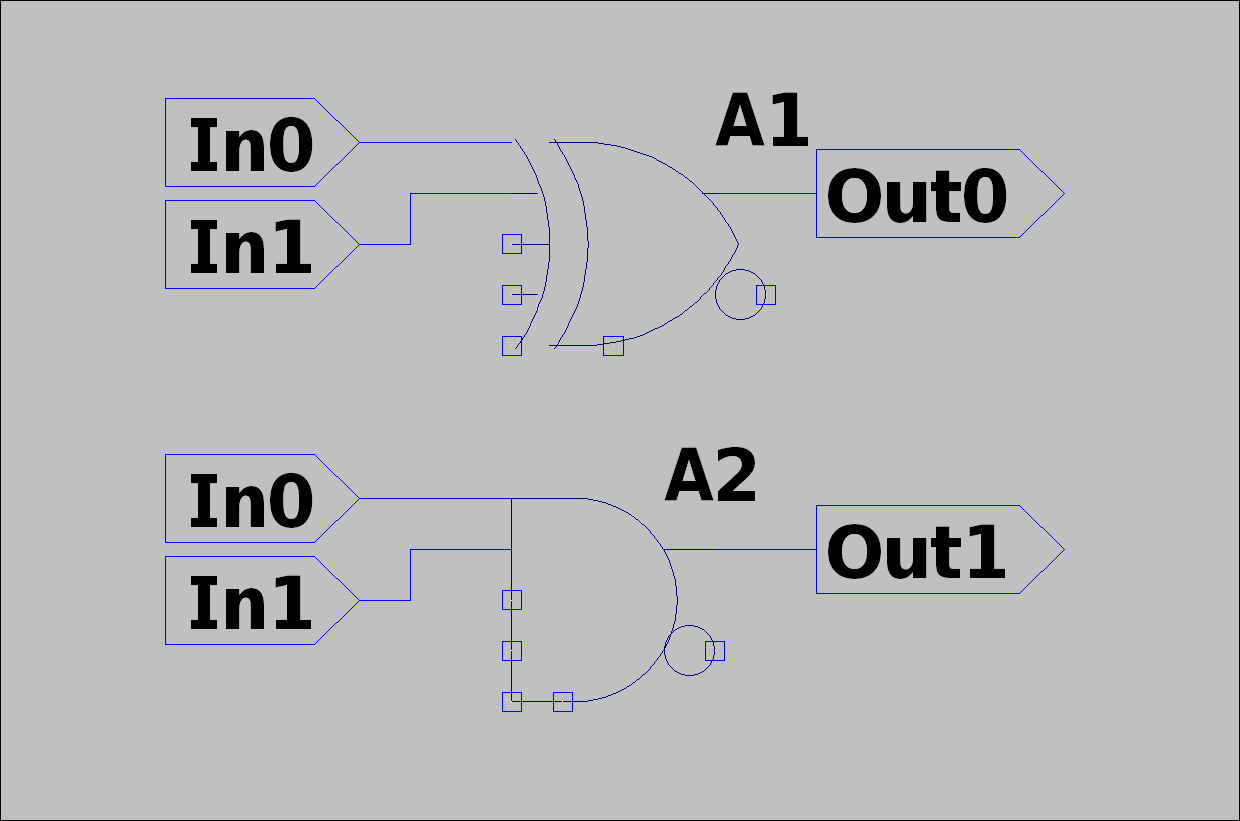
\includegraphics[width=\linewidth]{figures/half-adder.png}
        \caption{Half-adder circuit. Takes two 1-bit inputs and sums them to a 2-bit output.}
    \end{subfigure}
    \hfill
    \begin{subfigure}{0.45\linewidth}
        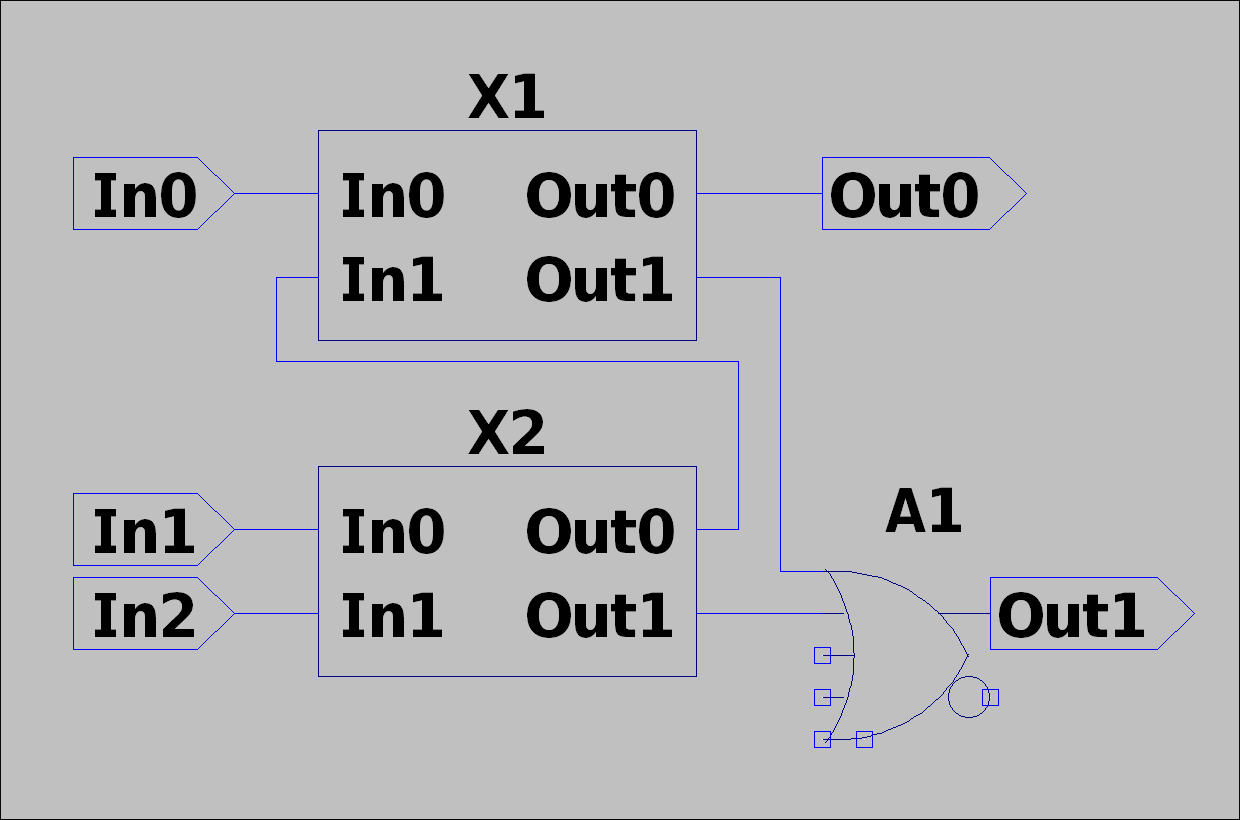
\includegraphics[width=\linewidth]{figures/full-adder.png}
        \caption{Full-adder circuit. Takes three 1-bit inputs and sums them to a 2-bit output.}
    \end{subfigure}
    \hfill
    \caption{Self-contained adder circuits used for simplifying the schematic for the multiplier circuit.}
    \label{fig:adders}
\end{figure}

In our actual circuit, we will not use any prefabricated half-adder or full-adder circuits. We will only use elementary logic gates for constructing the internal circuit. If we follow our current design, this will be done using only OR, XOR, and AND gates.

\begin{figure}[htb]
    \centering
    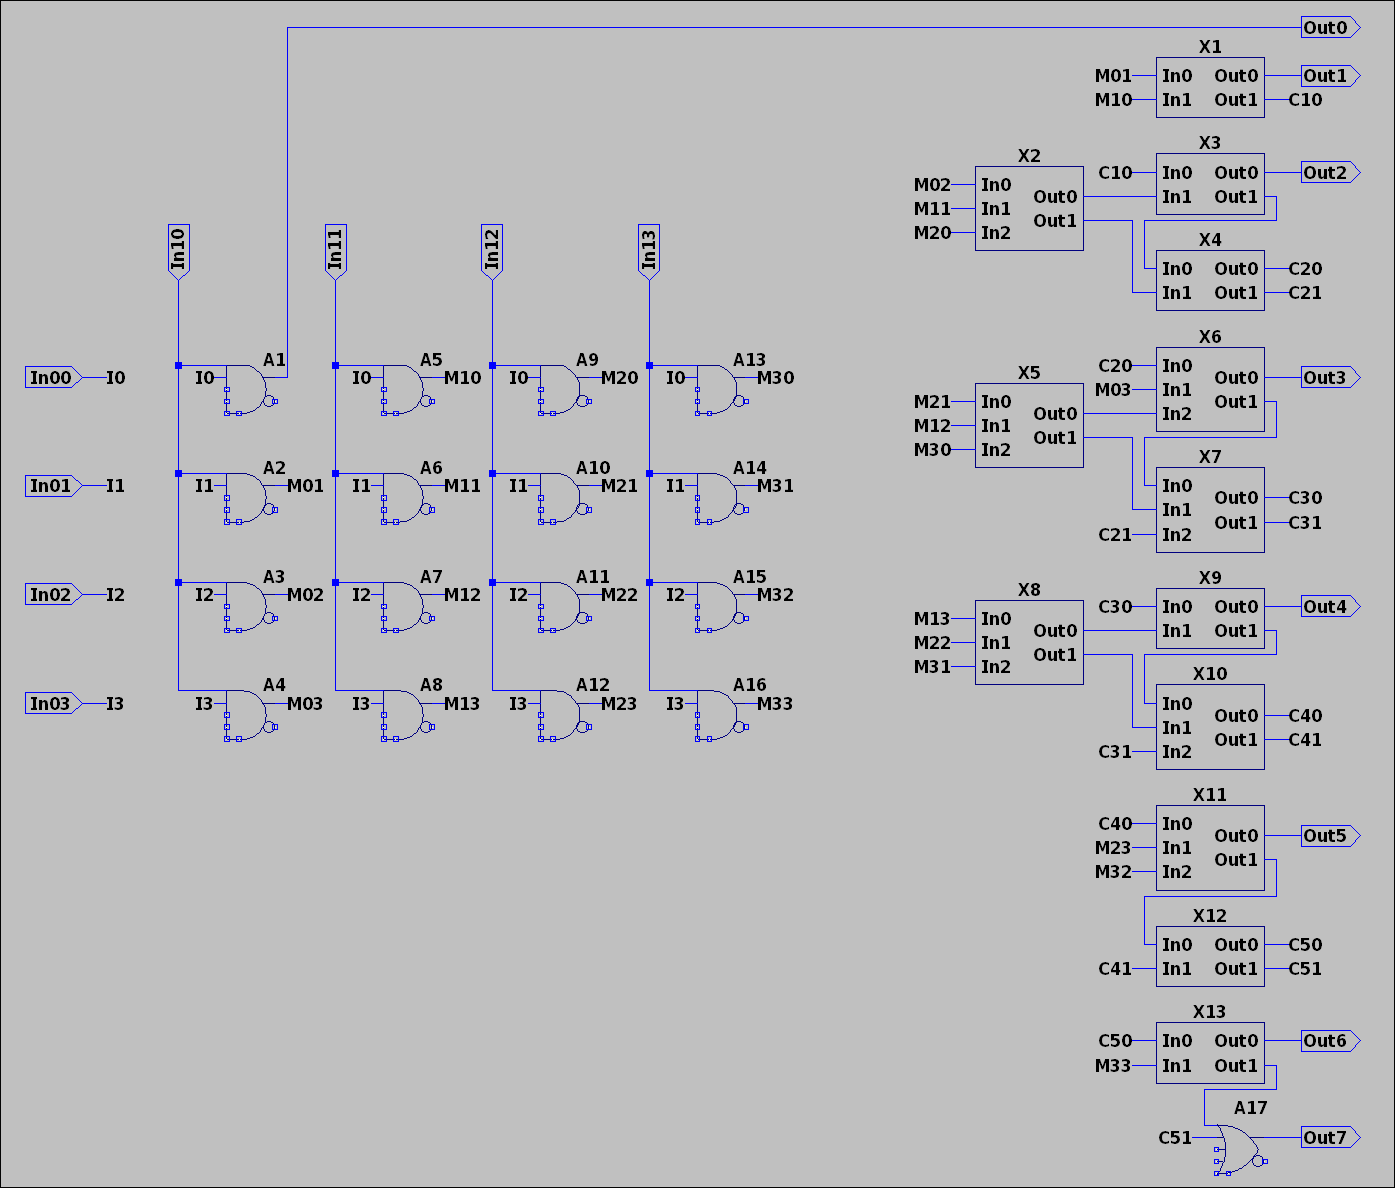
\includegraphics[width=0.8\linewidth]{figures/multiplier.png}
    \caption{Multiplier circuit schematic designed using half- and full-adder gates. Takes two 4-bit inputs and multiplies them to an 8-bit output.}
    \label{fig:multiplier}
\end{figure}

With this, our internal circuit's design can be seen in \autoref{fig:multiplier}. The first part of this circuit consists of a matrix of AND gates. In essence, what it's doing is that it's taking each digit of the input 1 and multiplying by input 0. So the first column is $I_{0*}\times I_{10}$, the second is $I_{0*}\times I_{11}$, and so on. The results from this multiplication are saved into MXX.

The next section of the circuit then adds these four numbers. This starts out simple, since M00 maps directly to Out0 (we had to connect it directly otherwise LTSpice wouldn't run our simulation). While the mini-circuit for each subsequent output is unique, they all share the same general design of (1) adding all the corresponding digits using a mix of adders, (2) determining what the OutX should be, and (3) what to carry over. The carry CXX is itself a binary number, most often 2-bit. The final output only has an OR gate because X13-Out1 and C51 are never high simultaneously, but they can be individually.

While the final result does require 8 bits to store, the largest it can be is only $15\times 15 = 225$.

\subsection{Interfacing with the Circuit}
To interface with the circuit, we will install two dip switches and seven digits of 7-segment displays. The dip switches are dials which output binary numbers from 0 to 15 and will act as our input. Given that both our inputs and outputs are binary numbers, we decided that it will be most straightforward to use a single Arduino to read the binary numbers and output each to 7-segment displays. We explored the option to use binary-to-BCD converters and related ICs, but ultimately using a single Arduino seemed easier and more cost-efficient.\footnote{Most of the ICs are only sold bulk, costing as much as \$300, and have very long delivery times. Since these are all specialized components anyway, we felt that there's no objective reason to use them over an Arduino.} The Arduino will read each of the inputs, as well as the output, and using a script (which we will write) convert the binary data to seven digits of 7-segment displays.

\section{Parts}
\subsection{Core Circuit}
Counting the gates in the internal circuit, we find that we will utilize 8 OR gates, 20 XOR gates, and 36 AND gates. If we were to use quad-chips like those we have already been using in labs, this would be at least 2 OR chips, 5 XOR chips, and 9 AND chips.\footnote{It might be more convenient to put separation between some of these chips, hence why ``at least''.} If we'd need to purchase all these gates ourselves, we could pick up \href{https://www.digikey.com/en/products/detail/texas-instruments/SN74HC32N/277235}{SN74HC32N}, \href{https://www.digikey.com/en/products/detail/texas-instruments/SN74HC86N/376842}{SN74HC86N}, and \href{https://www.digikey.com/en/products/detail/texas-instruments/SN74HC08N/277216}{SN74HC08N}.

\subsection{Interface}
The first part we'd need is the dip switch. After browsing DigiKey for a bit, we found that \href{https://www.digikey.com/en/products/detail/apem-inc/PT65503/1797077}{PT65503} looks to suit our needs well---we would get two of these. Then we'd need our 7-segment displays. Since we've got two inputs 0-15 and one output 0-225, we want two 2-digit displays and one 3-digit display. It seems like \href{https://www.digikey.com/en/products/detail/liteon/LTD-2701JD/3199020}{LTD-2701JD} and \href{https://www.digikey.com/en/products/detail/liteon/LTC-4724JR/408218}{LTC-4724JR} can do the job well. To power these displays, we'd also use some of the resistors available in the lab.

We have $2\times 4 + 8 = 16$ bits of binary and $7\times 7 = 49$ LED segments. Technically, due to the limited digits displayed in the largest position on each display (blank or one for 2-digit, blank, one, or two for 3-digit), we can exclude at least 11 segments. With this, we need an Arduino with at least $16+38=54$ pins. From looking it up online, an Arduino Mega should be sufficient. For example, \href{https://www.digikey.com/en/products/detail/arduino/A000067/2639006}{A000067}.

\subsection{Bill of Materials}
If we were to purchase all the components new, you can see the total costs in \autoref{fig:bom}. All items that we've picked out are available directly from DigiKey.
\begin{figure}[h]
    \centering
    \csvautotabular{bom.csv}
    \caption{Bill of materials. Most items listed will not have spares. The subtotal is \$98.41, or \$113.24 with shipping and tax.}
    \label{fig:bom}
\end{figure}

\end{document}
